\documentclass[12pt, 
hyperref={colorlinks=true, linkcolor=blue, urlcolor=cyan}]{beamer}
\usetheme{default} 

\setbeamertemplate{navigation symbols}{} %gets rid of navigation symbols
\setbeamertemplate{footline}{} %gets rid of bottom navigation bars
\setbeamertemplate{footline}[page number]{} %use this for page numbers

\setbeamertemplate{itemize items}[circle] %round bullet points
\setlength\parskip{10pt} % white space between paragraphs

\usepackage{comment}
\usepackage{wrapfig}
\usepackage{subfig}
\usepackage{setspace}
\usepackage{enumerate}
\usepackage{graphicx}
\usepackage{amsmath}
\usepackage{amsfonts}
\usepackage{amssymb}
\usepackage{amsthm}
\usepackage[UKenglish]{isodate}
\cleanlookdateon

% the preamble
\title{BIOST 311: \\ Regression Methods for the Health Sciences}
\author{Kelsey Grinde and Brian Williamson}
\institute{UW Biostatistics}
\date{Spring 2018}

\begin{document}
% title slide
\begin{frame}
\titlepage\thispagestyle{empty}
\end{frame}

% make it 2.something
\setbeamertemplate{footline}{%
  \raisebox{5pt}{\makebox[\paperwidth]{\makebox[120pt]{\scriptsize Last updated \today}\hfill\makebox[10pt]{\scriptsize 2.\insertframenumber~~}}}}  \newcounter{chap1}{\value{1}}
\setcounter{framenumber}{\value{chap1}}

\begin{frame}
\frametitle{CHAPTER 2: LOGISTIC REGRESSION}

By the end of Chapter 2, you should be able to:
\begin{itemize}
\item Distinguish between probability and odds and know how to calculate each in \texttt{R}
\item Formulate a regression model, given a scientific or statistical question about a binary outcome
\item Interpret the coefficients for a (simple or multiple) linear or logistic regression model with a binary outcome
\item Interpret confidence intervals and p-values for logistic regression coefficients
\item Describe how (and why) logistic regression interpretation changes when we have data from a case-control study
\item Use \texttt{R} to fit a logistic regression model  and to create figures/tables to support your logistic regression analysis
\end{itemize}
\end{frame}

\section{Binary outcomes}
\begin{frame}
\frametitle{SECTION 1: BINARY OUTCOMES}
Up to this point, we've focused on questions involving \textcolor{blue}{quantitative} outcomes:

\begin{itemize}
\item Is lung function (\textcolor{blue}{FEV}) associated with smoking?
\item Is lung function (\textcolor{blue}{FEV}) associated with smoking, after adjusting for age, height, and sex?
\item Does the association between lung function (\textcolor{blue}{FEV}) and smoking, adjusting for age and height, differ between males and females?
\item Is \textcolor{blue}{systolic blood pressure} associated with ancestry?
\item Is cognitive function (\textcolor{blue}{DSST score}) associated with alcohol use, adjusting for age, sex, and education?
\end{itemize}
\end{frame}

% binary outcome examples
\begin{frame}
\frametitle{SECTION 1: BINARY OUTCOMES}
However, we are often interested in questions that involve \textcolor{blue}{binary} outcomes:

\begin{itemize}
\item Are \textcolor{blue}{surgery complications} after upper endoscopy associated with who performed your sedation (anesthesiologist vs nurse)? % my work
\item Is \textcolor{blue}{cervical cancer} associated with hormonal contraceptive use? % group project
\item Is \textcolor{blue}{death from heart disease} associated with smoking?
\item Is \textcolor{blue}{diabetes} associated with sex? with age? % infarcts data
\end{itemize}
\end{frame}

% look at diabetes vs sex example
\begin{frame}
\frametitle{Example: diabetes and sex}

\begin{enumerate}
\item \textbf{Scientific Question:} is diabetes associated with sex?  \pause
\item \textbf{Statistical Question:} what do we mean by \textcolor{orange}{\textit{associated}}?  \pause
\end{enumerate}

There are multiple ways that we could check if diabetes is \textit{associated} with sex... \pause
\begin{itemize}
\item[] $p_M \stackrel{?}{=} p_F$ \textcolor{blue}{(probs)} \quad \quad \quad \quad \pause $\frac{p_M}{1-p_M} \stackrel{?}{=} \frac{p_F}{1-p_F}$ \pause \textcolor{blue}{(odds)} \pause
\item[] $p_M - p_F \stackrel{?}{=} 0$ \pause \textcolor{blue}{(RD)} \pause \quad \quad \quad $\frac{p_M}{1-p_M} - \frac{p_F}{1-p_F} \stackrel{?}{=} 0$ \pause
\item[] $p_M \div p_F \stackrel{?}{=} 1$ \pause \textcolor{blue}{(RR)} \pause \quad \quad \quad  $\left(\frac{p_M}{1-p_M}\right) \div \left(\frac{p_F}{1-p_F}\right) \stackrel{?}{=} 1$ \pause \textcolor{blue}{(OR)}
\end{itemize}
\end{frame}


% defining associations
\begin{frame}
\frametitle{Association}
When figuring out how we want to define \textit{association}, there are two parts that we need to think about...  \vspace{-0.3cm} \pause

\begin{itemize}
\item \textcolor{blue}{Summary measure}: probability, odds, mean
\item \textcolor{orange}{Contrast}: difference, ratio
\end{itemize} \pause

Examples: \vspace{-0.3cm}
\begin{itemize}
\item Is FEV associated with smoking? \pause
	\begin{itemize}
	\item[] $\rightarrow$ Is there a \textcolor{orange}{difference} in \textcolor{blue}{average} FEV between smokers and nonsmokers? \pause
	\end{itemize}
\item Is diabetes associated with sex? \pause
	\begin{itemize}
	\item[] $\rightarrow$ Is there a \textcolor{orange}{difference} in \textcolor{blue}{probability} of diabetes between men and women? \pause
	\item[] $\rightarrow$ Does the \textcolor{orange}{ratio} of \textcolor{blue}{odds} of diabetes between men and women differ from 1? %\pause \begin{tiny}(Note how awkward it is to talk about ratios ``in English")\end{tiny}
	\end{itemize}
\end{itemize}
\end{frame}

% diabetes and sex: linear regression
\begin{frame}
\frametitle{Example: diabetes and sex}

\begin{enumerate}
\item \textbf{Scientific Question:} is diabetes \textcolor{orange}{associated} with sex? \pause
\item \textbf{Statistical Question:} is there a \textcolor{orange}{difference in probability} of diabetes between men and women? \pause
	\begin{itemize}
	\item \textbf{Parameter:} difference in probabilities (or \textit{risk difference}) \pause
	\end{itemize}
\item Take a \textbf{sample} from the population: cohort study of adults aged 65 and older from 4 US communities \pause
\item Perform \textit{statistical inference}:
	\begin{itemize}
	\item Calculate a corresponding \textbf{statistic}: difference in probabilities in our sample
	\item Quantify uncertainty in your statistic
	\item Perform a hypothesis test \pause
	\end{itemize}
\end{enumerate}

We can use linear regression to answer this question!
\end{frame}

% aside: mean of a binary variable
\begin{frame}
\frametitle{Linear regression with a binary outcome}

Simple linear regression model: $$E[Y \mid X] = \beta_0 + \beta_1 X$$

$E[Y \mid X]$ is the \textcolor{blue}{\textit{expected value}} of $Y$ given $X$ (or the \textcolor{blue}{\textit{average}}) \pause

What's the average of a binary variable $Y$? \pause \textit{It's the probability that $Y$ equals 1!} $\left(\text{i.e., } E[Y] = \text{P}(Y=1)\right)$ \pause

\begin{itemize} \itemsep +12pt
\item[] $Y = \{ 0, 0, 1, 0, 1, 1, 0, 0, 1, 1 \}$ \pause
\item[] $\bar{Y} = \frac{0 + 0 + 1 + 0 + 1 + 1 + 0 + 0 + 1 + 1}{10} = \frac{1}{2}$ \pause
\item[] $\hat{p} = \widehat{\text{P}(Y=1)} = \frac{5}{10} = \frac{1}{2} $
\end{itemize}
\end{frame}

% activity: interpret lin reg coefficients
\begin{frame}
\frametitle{Activity: diabetes and sex}

Suppose we fit the linear regression model $$E[diabetes \mid male] = \beta_0 + \beta_1 male,$$ \begin{footnotesize}where $diabetes = 1$ if diabetes and $diabetes = 0$ if no diabetes, \\ and $male = 1$ if male and $male = 0$ if female. \end{footnotesize}

\color{blue} On a piece of paper, please answer the following questions: 

\begin{enumerate}
\item \color{blue} Interpret the intercept, $\beta_0$.
\item Interpret the slope, $\beta_1$.
\end{enumerate} \color{black}

(You will turn this in at the end of class.)
\end{frame}

% linear regression: diabetes vs sex
\begin{frame}
\frametitle{Linear regression: diabetes vs sex}

Suppose we fit the linear regression model $$E[diabetes \mid male] = \beta_0 + \beta_1 male$$

How do we interpret the regression coefficients $\beta_0, \beta_1$? \vspace{-0.3cm}

\begin{itemize}
\item \color{blue} $\beta_0$: \pause the probability of diabetes among females \pause \color{black}
\item[] \ \ \begin{scriptsize} (the average value of diabetes among females) \end{scriptsize} \pause
\item \color{blue} $\beta_1$: \pause the difference in probability of diabetes between males and females \pause \color{black}
\item[] \ \ \begin{scriptsize}(the difference in average value of diabetes between males and females) \pause \end{scriptsize}
\end{itemize}

\vspace{-0.3cm}
To answer our statistical question \begin{small}\textit{(is there a difference in probability of diabetes between men and women?)}\end{small} we just need to look at $\beta_1$! \begin{small} (estimate, CI, test if it's equal to 0) \end{small}
\end{frame}

% motivate logistic regression
\begin{frame}
\frametitle{Diabetes vs sex: odds}
\begin{small} What if we wanted to quantify the association between diabetes and sex via the \textit{odds ratio} rather than the \textit{risk difference}? \end{small} \pause

\vspace{-0.3cm}

\begin{enumerate}
\item \textbf{Scientific Question:} is diabetes \textcolor{orange}{associated} with sex? \pause
\item \textbf{Statistical Question:} is the \textcolor{orange}{ratio of odds} of diabetes between men and women different from 1? \pause
	\begin{itemize}
	\item \textbf{Parameter:} odds ratio \pause
	\end{itemize}
\item Take a \textbf{sample} from the population: cohort study of adults aged 65 and older from 4 US communities \pause
\item Perform \textit{statistical inference}:
	\begin{itemize}
	\item Calculate a corresponding \textbf{statistic}: sample odds ratio
	\item Quantify uncertainty in your statistic
	\item Perform a hypothesis test \pause
	\end{itemize}
\end{enumerate}

\vspace{-0.4cm}
We can use \textcolor{blue}{logistic} regression to answer this question!
\end{frame}

% ask them to think about logistic regression interp
\begin{frame}
\frametitle{Activity (continued): diabetes vs sex}
Suppose we fit the logistic regression model $$\log\left(\text{Odds}[diabetes | male]\right) = \beta_0 + \beta_1 male$$

\color{blue} On the same piece of paper, please answer these questions:

\begin{enumerate}
\item[3.] \color{blue} Interpret the intercept, $\beta_0$.
\item[4.] Interpret the slope, $\beta_1$.
\end{enumerate}
\end{frame}

% logistic regression: diabetes vs sex
\begin{frame}
\frametitle{Logistic regression: diabetes vs sex}

Suppose we fit the logistic regression model $$\log\left(\text{Odds}[diabetes | male]\right) = \beta_0 + \beta_1 male$$

\vspace{-0.2cm}

How do we interpret the regression coefficients $\beta_0, \beta_1$? \vspace{-0.3cm}
\begin{itemize}
\item $\beta_0$: \pause the log odds of diabetes among females \pause
\item[] \color{blue} $e^{\beta_0}$: the odds of diabetes among females \pause \color{black}
\item $\beta_1$: \pause the difference in log odds of diabetes between males and females \pause 
\item[] \color{blue} $e^{\beta_1}$: the ratio of odds between males and females \color{black}
\end{itemize}

\vspace{-0.2cm}
To answer our statistical question \begin{small}\textit{(is the ratio of odds of diabetes between men and women different from 1?)}\end{small} we just need to look at $e^{\beta_1}$! \begin{small} (estimate, CI, test if it's equal to 1) \end{small}
\end{frame}

\begin{frame}
The interpretation of logistic regression models is
\begin{itemize}
\item[] \color{blue} more complicated \color{black} (we have to remember to exponentiate the coefficients, and to talk about ratios rather than differences), and
\item[] \color{orange} less intuitive \color{black} (a lot of people don't understand the difference between probabilities and odds)...
\end{itemize}
\textit{so why bother?}
\end{frame}

\section{Linear regression with binary outcomes}
\begin{frame}
\frametitle{SECTION 2: LINEAR REGRESSION WITH BINARY OUTCOMES}

Linear regression model with a binary outcome: $$E[Y|X_1,\cdots,X_p] = \beta_0 + \beta_1 X_1 + \beta_2X_2 + \cdots \beta_p X_p$$ $$P[Y=1|X_1,\cdots,X_p] = \beta_0 + \beta_1 X_1 + \beta_2 X_2 + \cdots \beta_p X_p$$

Interpretation:
\begin{itemize}
\item $\beta_0$: probability that $Y=1$ when $X_1 = 0, \cdots X_p = 0$
\item $\beta_1$: difference in probability that $Y=1$ comparing two groups that differ by one unit in $X_1$ but are the same with respect to $X_2,\cdots,X_p$ 
\item ...
\end{itemize}
\end{frame}

\begin{frame}
\frametitle{Linear regression with binary outcomes}
\begin{center} $E[Y|X_1,\cdots,X_p] = \beta_0 + \beta_1 X_1 + \beta_2 X_2 + \cdots \beta_p X_p$ \end{center}

\vspace{-0.6cm}
\color{blue} Inference: \vspace{-0.3cm} \color{black}
\begin{itemize}
\item Identify the regression coefficient of interest, $\beta$. \pause % which one(s) answer(s) our scientific Q?
\item Report an estimate of $\beta$, and interpret: \textit{We estimate that the difference in probabilities between two groups...} \pause
\item Report a 95\% confidence interval for $\beta$, and interpret: \textit{Based on a 95\% confidence interval, this observed difference in probabilities would not be judged unusual if...} \pause
\item Report the p-value from a hypothesis test of $H_0: \beta = 0$: \textit{These data provide evidence to suggest that this difference in probabilities is (is not) significantly different from zero ($p =$...).} \pause
\item Add a conclusion relating back to our scientific question
\end{itemize}
% they'll fill in the blanks on HW this week
\end{frame}

\begin{frame}
\frametitle{Linear regression with binary outcomes}
\begin{center} $E[Y|X_1,\cdots,X_p] = \beta_0 + \beta_1 X_1 + \beta_2 X_2 + \cdots \beta_p X_p$ \end{center}

\color{blue} Prediction:\vspace{-0.3cm} \color{black}
\begin{itemize} \itemsep +5pt
\item Get estimates for each regression coefficient: $\hat\beta_0, \cdots, \hat\beta_p$ \pause
\item Plug in those estimates, along with the covariate values for the new individual: $\hat\beta_0 + \hat\beta_1 x_1 + \cdots \hat\beta_p x_p$ \pause
	\begin{itemize} \itemsep +5pt
	\item This is our best estimate of $Y$ for a person with $X_1 = x_1, \cdots X_p = x_p$ ($\hat{Y}$) \pause
	\item This is also our estimate of the mean value of $Y$ (or probability that $Y=1$) among subjects with $X_1 = x_1, \cdots, X_p = x_p$ ($\hat{E}[Y|X_1,\cdots X_p] = \hat{P}[Y=1|X]$)
	\end{itemize}
\end{itemize}

\end{frame}

\begin{frame}
\frametitle{Linear regression with binary outcomes}
\begin{center} $E[Y|X_1,\cdots,X_p] = \beta_0 + \beta_1 X_1 + \beta_2 X_2 + \cdots \beta_p X_p$ \end{center}

\color{blue} Graphical support: \color{black} scatterplot + linear regression line
\vspace{-0.4cm}
\center
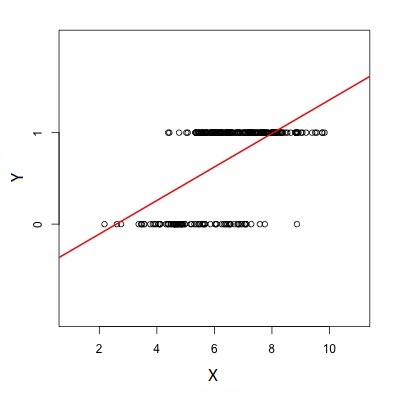
\includegraphics[width=0.5\textwidth]{figs/contX-lm}
\end{frame}

\begin{frame}[noframenumbering]
\frametitle{Linear regression with binary outcomes}
\begin{center} $E[Y|X_1,\cdots,X_p] = \beta_0 + \beta_1 X_1 + \beta_2 X_2 + \cdots \beta_p X_p$ \end{center}

\color{blue} Graphical support: \color{black} \textit{What is $\hat{Y}$ for someone with $X = 10$?}
\vspace{-0.4cm}
\center
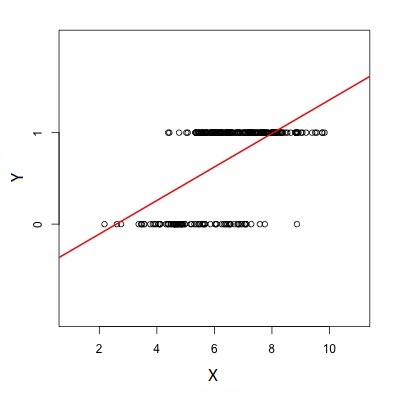
\includegraphics[width=0.5\textwidth]{figs/contX-lm}
\end{frame}


\begin{frame}
\frametitle{Linear regression with binary outcomes}
\begin{center} $E[Y|X_1,\cdots,X_p] = \beta_0 + \beta_1 X_1 + \beta_2 X_2 + \cdots \beta_p X_p$ \end{center}

Pros: \vspace{-0.3cm}
\begin{itemize}
\item Easy to interpret (differences in probabilities)
\end{itemize}

Cons: \vspace{-0.3cm}
\begin{itemize}
\item Predicted/fitted values can be outside the (0,1) range
\item Our mean model might not be correct (particularly the linearity piece)% is one of the assumptions for linear regression that actually is important
\end{itemize}

What can we do instead?
\end{frame}

\section{Simple logistic regression}
\begin{frame}
\frametitle{SECTION 3: SIMPLE LOGISTIC REGRESSION}

% motivation: keep things between 0 and 1
% general formulation, do the math for coefficient interp
% relate to a glm (explain logit function)
% diabetes and sex: logistic regression; interp + R + reporting results; back transforming to get probs
% diabetes and sex: chi-squared test [put this on HW?]; interp + R + reporting results
% diabetes and age: interp + R + reporting results

\end{frame}


%%%%%%%%%%%%%%%%%%%%% comment out %%%%%%%%%%%%%%%%%%%
\begin{comment}

\section{Multiple logistic regression}
\begin{frame}
\frametitle{SECTION 4: MULTIPLE LOGISTIC REGRESSION}
\end{frame}

\section{Relative risk regression}
\begin{frame}
\frametitle{Relative risk regression}
It exists!
% mention relative risk regression: log(E[Y|X]) = b0 + b1X
\end{frame}

\section{Summary of regression methods for binary outcomes}
\begin{frame}
\frametitle{Summary}
%% summary: come back to slide 2.4 and highlight which type of regression answers which statistical question
\end{frame}

\section{Logistic regression in case-control studies}
\begin{frame}
\frametitle{SECTION 5: LOGISTIC REGRESSION IN CASE-CONTROL STUDIES}
\end{frame}

% prediction?
%\section{Prediction}

% assumptions/diagnostics?
%\section{Assumptions and diagnostics}

\end{comment}


\end{document}
